\chapter{Analyze}

\section{Environments}
Two environments are developed for comparing the \gls{drl} algorithms used in this thesis: single-agent bilateral negotiation environment (\gls{sbe}) and multi-agent concurrent bilateral negotiation environment (\gls{mcbe}). The details are described in section \ref{single-agent-env} and \ref{multi-agent-env}. In addition to these environments, some methods have been implemented to make the training logic clearer, such as \texttt{Game} in section \ref{game} and \texttt{Scenario} in section \ref{scenario}.

\section{\gls{negmas} with \gls{openai gym}}
\gls{negmas} has implemented some negotiation mechanisms and specific simulated world, such as \gls{saom} and \gls{scml} (Now as an independent project). In order to compare the algorithms in specific simulated world more easily, an interface is needed to connect \gls{negmas} and \gls{rl} algorithms. This interface and all algorithms can be rewritten from scratch, but it is very time-consuming and not ideal. The second option is to implement some RL framework interfaces, which will reduce a lot of work. OpenAI realize the environmental standardization and comparison of algorithms with the help of toolkit \gls{openai gym} \parencite{brockman2016openai}. Although \gls{openai gym} is not enough to complete the work in this thesis, the baseline algorithms and the environmental interface in the package greatly speed up the work. In this section, the implementation of environment and assisted methods used in bilateral negotiation will be presented.

With the help of \gls{openai gym},  a bilateral negotiation environment can be developed on the top of \gls{saom} to research reinforcement learning algorithms. \gls{openai gym} implements many baseline algorithms, which can be easily tested in a custom environment.

\subsection{Negotiation Issues}
\gls{negmas} provoides some classes and methodes to design issues flexibly. In \gls{sbe} following issues are used:
 
\paragraph{Price} Integer between two values, such as (10, 20)
\paragraph{Quantity} Integer between two values, such as (1, 10)
\paragraph{Time} Relative step between zero and maximal step.

\subsection{Model}
The model consists of five parts, environment \texttt{\gls{sbe}}, negotiation game, negotiation mechanism, negotiator and reinforcement learning algorithms.
Except for the negotiation mechanism mentioned and implemented in sections \ref{autonomous-negotiation} and \ref{background:negmas}, others parts will be introduced step by step in following sections. 

Entire model is shown in \ref{fig:environment-single-agent}.
\begin{figure}[htbp]
\centering
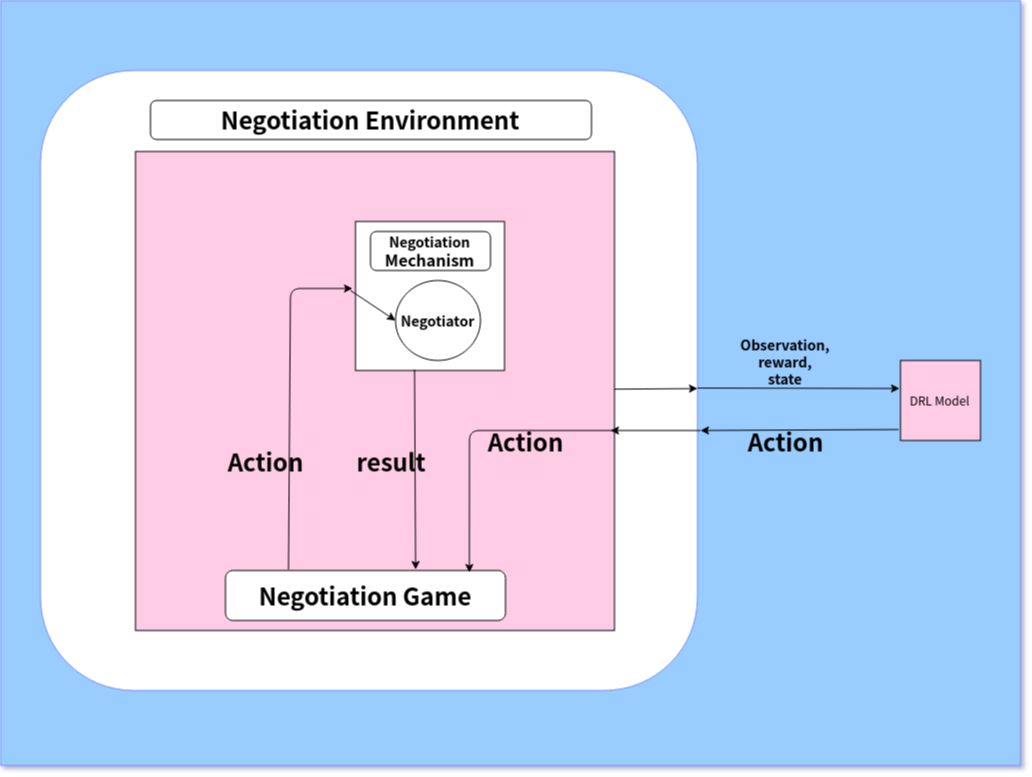
\includegraphics[width=0.60\textwidth]{./images/environment-single-agent.png}
\caption{Environment for single agent bilateral negotiation based on NegMAS}
\label{fig:environment-single-agent}
\end{figure}

\subsection{Single-Agent Environment} \label{single-agent-env}
The interface of the OpenAI Gym Environments is designed for one agent as standard. Nevertheless, it must be examined how the \gls{sbe} can be represented via this interface and controlled by the controller. The methods of the interface for the \gls{sbe} are therefore defined below. 

\paragraph{STEP} Firstly, set up but not perform the action received from \gls{rl} model for the negotiator. Then, run the negotiation mechanism (such as \gls{saom} ) for one step. All actions will be perfomed by the negotiation mechanism. Finally, the function returns four parameters.

\begin{itemize}
	\item Observation: Offer proposed by opponent and current realitive time.
	\item Reward: Utility value of the current offer and extra reward when an agreement is reached.
	\item Done: Reach the final state or there is no agreement within the maximum running time.
	\item Info: State of the negotiation mechanism, extra info used for evaluation.
\end{itemize}

\paragraph{RESET} Resets the environment(SBE) and other related parameters(in Game) to an initial state after every episode and returns an initial observation.
\paragraph{RENDER} Define how to display the output of the environment. Multiple modes can be used: 

\paragraph{CLOSE}
\paragraph{SEED}

\subsection{Game} \label{game}
In addition to implementing the official \gls{openai gym} \texttt{Env} interface, class Game is designed to control the entire negotiation mechanism. The purpose of this design is to reduce the modification of negotiatioin mechanism of \gls{negmas}.

\paragraph{STEP}

\subsection{Challenges of the environment}

\subsection{Analysis of the reinforcement learning algorithms}

\subsection{Conclusion}


\section{\gls{scml} with \gls{openai gym}}
\subsection{Multi-Agent Environment} \label{multi-agent-env}

Official api methods, and add new method \texttt{run} to run one episode.

\paragraph{Step:}
\paragraph{RESET:}
\paragraph{CLOSE:}
\paragraph{SEED:}

\subsection{Scenario} \label{scenario}

\subsection{Challenges of the environment}
Combination with \gls{negmas}

\subsection{Analysis of the reinforcement learning algorithms}

\subsection{Conclusion}
